\documentclass [11pt, a4wide, twoside]{article}

\usepackage{times}
\usepackage{epsfig}
\usepackage{ifthen}
\usepackage{xspace}
\usepackage{fancyhdr}
\usepackage{moreverb}
\usepackage{amsmath}
\usepackage{amsthm}
\usepackage[usenames, dvipsnames]{color}
\usepackage{stmaryrd}
\usepackage[colorlinks=true, urlcolor = blue, linkcolor=blue]{hyperref}
\usepackage{listings}
\usepackage{color}
% solution switch
\newboolean{showsolution}
\setboolean{showsolution}{true}


%layout
\topmargin      -5.0mm
\oddsidemargin  6.0mm
\evensidemargin -6.0mm
\textheight 215.5mm
\textwidth      160.0mm
\parindent        1.0em
\headsep          10.3mm
\headheight        12pt
\lineskip    1pt
\normallineskip     1pt

%header
\lhead{Programming Languages \\ 2021}

\rhead{Prof. O. Nierstrasz\\
Mohammadreza Hazhirpasand, Joel Niklaus}
\lfoot{page \thepage}
\rfoot{\today}
\cfoot{}

\renewcommand{\headrulewidth}{0.1pt}
\renewcommand{\footrulewidth}{0.1pt}

\renewcommand{\thesubsection}{\arabic{subsection}}

%enumeration
\newenvironment{myitemize}{%
     \begin{itemize}
     \setlength{\itemsep}{0cm}}
     {\end{itemize}}

\newenvironment{myenumerate}{%
     \begin{enumerate} \setlength{\itemsep}{0cm}}
     {\end{enumerate}}


%solution
\ifthenelse{\boolean{showsolution}}
   {  \newcommand{\solution}[1]{
   	\noindent\underline{\textbf{Answer:}}\\[2mm]
   	 \textsl{#1}
	 \vspace{10pt}
	 \normalsize
	}
  }
  {  \newcommand{\solution}[1]{} }

\newcounter{exnum}
\def\xexercise{\fontsize{12}{10}\fontseries{bx}\selectfont}
\def\xnormal{\fontseries{m}\fontshape{n}\selectfont}


\newcommand{\exercise}[1]{%
     {\addtocounter{exnum}{1}\vskip 0.8cm{\xexercise \noindent Exercise
\arabic{exnum} (#1)} \xnormal} \vskip 0.3cm} 
 \newcommand{\aufgabe}[1]{
     {\addtocounter{exnum}{1}\vskip 0.8cm{\xexercise \noindent Aufgabe
\arabic{exnum} (#1)} \xnormal} \vskip 0.3cm} 

\pagestyle{fancy}


% ===============ABBREVIATIONS==============================
\newcommand{\eg}{\emph{e.g.,}\xspace}
\newcommand{\ie}{\emph{i.e.,}\xspace}
\newcommand{\etc}{\emph{etc.}\xspace}


\begin{document}

% title
\section*{\ifthenelse{\boolean{showsolution}}{Solution }{}\xspace{}Objects and Prototypes}

\subsection*{Instructions:}

\textbf{Solutions of the exercises are to be delivered before Thursday, the 03th of May at 10:15AM.}\\
Solutions should be placed in a separate folder with the name ``\textbf{Assignment08}''.\\

% - - - - - - - - - - - - - - - - - - - - - - - - - - - - - - - - - - - - - - - - - - - - - - - - - - - - - - - - - - - - - - - - - - -
\subsection*{Exercise 1 (2 points)}

You should implement the \texttt{Person} prototype which has the following characteristics:

\begin{enumerate}
   \item The \texttt{name} property which is accessible by other objects of this prototype.
   \item The \texttt{password} property which cannot be accessed by other objects of this prototype.
   \item The \texttt{counter} property whose value is shared among all objects of this prototype.
 \end{enumerate}

You need to create two objects of this prototype in order to do the following tasks:

\begin{enumerate}
   \item Show how to access the \texttt{name} property in both objects.
   \item What output do you get if you try to access the \texttt{password} property? How can you correct it?
   \item How to access the \texttt{counter} property? If you change the value of the \texttt{counter} property in one object, does it affect the property value on the second object?
 \end{enumerate}

\vspace{0.5cm}

\solution{\texttt{factors :: Int -> [Int]}\\
since both \texttt{n} and \texttt{x} are arguments of the function \texttt{mod} which accepts only the \texttt{Int} arguments\\
\\
\texttt{isPerfect :: Int -> Bool}\\
since \texttt{n} is an argument of the function \texttt{factors} which accepts only the \texttt{Int} arguments,\\
and \texttt{== :: Eq a => a -> a -> Bool}\\
\\
Both functions are monomorphic.\\
\texttt{-----------------------------------------------------------------------}\\
\texttt{insert :: Int -> a -> [a] -> [a]}\\
since\\
\texttt{insert \_ n l = [n] => insert :: a->b->c->[b]}\\
\texttt{insert 0 n l = n:l => insert :: Int->b->[b]->[b]}\\
The \texttt{insert} function is polymorphic.

\texttt{mH (a, b, c) = c} \\

\texttt{mH :: (x, y, z) -> z}\\
mH is polymorphic since the three elements a, b, and c may be of any type. \\}




% - - - - - - - - - - - - - - - - - - - - - - - - - - - - - - - - - - - - - - - - - - - - - - - - - - - - - - - - - - - - - - - - - - -
\subsection*{Exercise 2 (2 points)}


A possible classification for animals is shown in Figure \ref{fig:ex2}. When it comes to classify the platypus you realize that it nurses but it also spawns. So implement the class diagram shown in figure \ref{fig:ex2} including the poor platypus in Java Script. Use the \href{http://scg.unibe.ch/download/lectures/pl2018-exercises/poorPlatypusToSolve.html}{poorPlatypusToSolve.html} file as skeleton for your implementation.

\begin{figure}[ht!]
\begin{center}
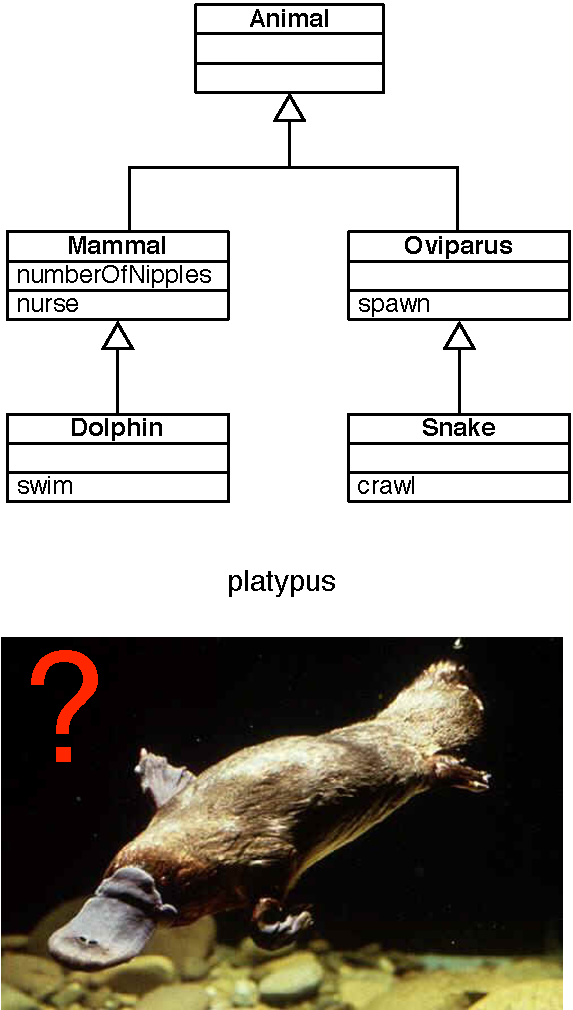
\includegraphics[width=0.4\columnwidth]{solutions/Ex2.pdf}
\caption{Animal classification}
\label{fig:ex2}
\end{center}
\end{figure}

\solution{\begin{verbatim}
<html>
<head>
<title>Platypus</title>
<script type="text/javascript">

var animal = {}

var mammal = Object.create(animal);
mammal.numberofNipples = 2;
mammal.nurse = function () {
	alert("I am nursing");
}
mammal.getNumberOfNipples = function(){
	alert(this.numberofNipples);
}

dolphin = Object.create(mammal);
dolphin.numberofNipples = 4;
dolphin.swim = function() {
	alert("I am swimming");
}

var oviparus = Object.create(animal);
oviparus.spawn = function() {
	alert("I am spawning");
}

var snake = Object.create(oviparus);
snake.crawl = function() {
	alert("I am crawling");
}

var platypus = Object.create(mammal);
platypus.numberofNipples = 6;
platypus.spawn = oviparus.spawn;

function display(text) {
	document.getElementById("output").innerHTML += text + "\n";
}

</script>
</head>
<body>
<pre id="output">
</pre>
<a href="#" onClick="mammal.getNumberOfNipples();">mammal's number of nipples</a> <br/><br/>

<a href="#" onClick="dolphin.swim();">dolphin swimming</a> <br/><br/>
<a href="#" onClick="dolphin.nurse();">dolphin's nursing</a> <br/><br/>
<a href="#" onClick="dolphin.getNumberOfNipples();">dolphin number of nipples</a> <br/><br/>


<a href="#" onClick="snake.crawl();">snake crawling</a> <br/><br/>
<a href="#" onClick="snake.spawn();">snake spawning</a> <br/><br/>

<a href="#" onClick="platypus.nurse();">platypus nursing</a> <br/><br/>
<a href="#" onClick="platypus.spawn();">platypus spawning</a> <br/><br/>
<a href="#" onClick="platypus.getNumberOfNipples();">platypus's number of nipples</a> <br/><br/>
</body>
</html>
\end{verbatim}

}


% - - - - - - - - - - - - - - - - - - - - - - - - - - - - - - - - - - - - - - - - - - - - - - - - - - - - - - - - - - - - - - - - - - -
\subsection*{Exercise 3 (2 points)}



In this exercise, the prototype \texttt{People} is defined. You need to define two objects of this prototype.
The first object must be created by the \texttt{Object.create()} method and the second object must be created by a constructor function.
Finally, to check if your solution is correct, run the \texttt{checkit} method from the \href{http://scg.unibe.ch/download/lectures/pl2018-exercises/Third-template.htm}{template}.
This method must return \texttt{Bern} in both objects.




\vspace{0.5cm}
\solution{\begin{verbatim}
var People = function () {
    this.username = "Bern";
	return this;
};

People.prototype.checkit = function() {
	return this.username;
}


var c = new People();
d = Object.create(People.prototype);

People.apply(d);

console.log(c.checkit());
console.log(d.checkit());
\end{verbatim}}

\end{document}
